\documentclass[UTF8]{book}
%\usepackage{ctex}
\usepackage{amsmath}
\usepackage{bm}
\usepackage{makeidx}
\usepackage{enumitem}
\usepackage{rotating} 
\usepackage{yhmath}
\usepackage{textcomp,booktabs}
\usepackage[usenames,dvipsnames]{color}
\usepackage{colortbl}
\usepackage{makecell}
\usepackage{gensymb}
\usepackage{cancel}
\usepackage{graphicx}
\usepackage{pifont}
\usepackage[all,pdf]{xy}
\usepackage{exscale}
\usepackage{blindtext}
\usepackage{hyperref}
\hypersetup{
colorlinks=true,
linkcolor=black
}
\usepackage{nameref}
\usepackage{relsize}
\usepackage{titlesec}
\usepackage{ifthen}
\usepackage{array}
\usepackage[flushleft]{threeparttable}
\usepackage{diagbox}
\usepackage{mathtools}
\usepackage{amsfonts}
\usepackage{bbm}
\usepackage{ulem}
\usepackage{xcolor}
\usepackage{color}
\usepackage{mathptmx}
\usepackage{amssymb}
\usepackage{geometry}
\geometry{a4paper, left=2.54cm,right=2.54cm,top=2.54cm,bottom=2.54cm}
%\geometry{b5paper, left=1.6cm,right=2cm,top=2cm,bottom=2cm}
\usepackage{mathrsfs}
\usepackage{tikz,tkz-euclide}
\usepackage{tikz}
\usetikzlibrary{patterns}
\usetikzlibrary{shapes,arrows}
\usepackage{esvect}
\usepackage{fancyhdr}
\pagestyle{fancy}
\fancyhead{} % clear all fields 
\cfoot{}
\fancyhead[LE,RO]{\thepage} 
\renewcommand{\headrulewidth}{0pt}
\renewcommand{\footrulewidth}{0pt}
\linespread{1.4}
\date{}
\graphicspath{ {Graphs} }
\usepackage{listings}
\usepackage{color}

\definecolor{dkgreen}{rgb}{0,0.6,0}
\definecolor{gray}{rgb}{0.5,0.5,0.5}
\definecolor{mauve}{rgb}{0.58,0,0.82}

\lstset{
  basicstyle=\ttfamily,
  columns=fullflexible,
  frame=single,
  breaklines=true,
  backgroundcolor=\color{gray!20!white}
}
\definecolor{codegray}{gray}{0.8}
\newcommand{\code}[1]{\colorbox{codegray}{\texttt{#1}}}
%通用:
\newcounter{mylabelcounter}
\makeatletter
\newcommand{\labeltext}[2]{%
#1\refstepcounter{mylabelcounter}%
\immediate\write\@auxout{%
  \string\newlabel{#2}{{1}{\thepage}{{\unexpanded{#1}}}{mylabelcounter.\number\value{mylabelcounter}}{}}%
}%
}
%Xsum
\DeclareFontFamily{U} {cmex}{}
\DeclareFontShape{U}{cmex}{m}{n}{
  <-6> cmex5
  <6-7> cmex6
  <7-8> cmex7
  <8-9> cmex8
  <9-10> cmex9
  <10-12> cmex10
  <12-> cmex12}{}
\DeclareSymbolFont{Xcmex} {U} {cmex}{m}{n}
\DeclareMathSymbol{\Xdsum}{\mathop}{Xcmex}{88}
\DeclareMathSymbol{\Xtsum}{\mathop}{Xcmex}{80}
\DeclareMathOperator*{\Xsum}{\mathchoice{\Xdsum}{\Xtsum}{\Xtsum}{\Xtsum}}
%Xsum
%choice
\newcommand{\fourch}[4]{%~\hfill(\qquad)\\
\begin{tabular}{*{4}{@{}p{0.25\textwidth}}}(A)~#1 & (B)~#2 & (C)~#3 & (D)~#4\end{tabular}}
\newcommand{\twoch}[4]{%~\hfill(\qquad)\\
\begin{tabular}{*{2}{@{}p{0.5\textwidth}}}(A)~#1 & (B)~#2\end{tabular}\\\begin{tabular}{*{2}{@{}p{0.5\textwidth}}}(C)~#3 & (D)~#4\end{tabular}}
\newcommand{\onech}[4]{%~\hfill(\qquad)\\
(A)~#1 \\ (B)~#2 \\ (C)~#3 \\ (D)~#4}
 
\newlength\widthcha
\newlength\widthchb
\newlength\widthchc
\newlength\widthchd
\newlength\widthch
\newlength\tabmaxwidth
\setlength\tabmaxwidth{1\textwidth}
\newlength\fourthtabwidth
\setlength\fourthtabwidth{0.25\textwidth}
\newlength\halftabwidth
\setlength\halftabwidth{0.5\textwidth}
\newcommand{\choice}[4]{\settowidth\widthcha{AM.#1}\setlength{\widthch}{\widthcha}
    \settowidth\widthchb{BM.#2}
    \ifthenelse{\widthch<\widthchb}{\setlength{\widthch}{\widthchb}}{}
    \settowidth\widthchb{CM.#3}
    \ifthenelse{\widthch<\widthchb}{\setlength{\widthch}{\widthchb}}{}
    \settowidth\widthchb{DM.#4}
    \ifthenelse{\widthch<\widthchb}{\setlength{\widthch}{\widthchb}}{}
    \ifthenelse{\widthch<\fourthtabwidth}{\fourch{#1}{#2}{#3}{#4}}
    {\ifthenelse{\widthch<\halftabwidth\and\widthch>\fourthtabwidth}{\twoch{#1}{#2}{#3}{#4}}
        {\onech{#1}{#2}{#3}{#4}}}}
%choice
% Default fixed font does not support bold face
\DeclareFixedFont{\ttb}{T1}{txtt}{bx}{n}{12} % for bold
\DeclareFixedFont{\ttm}{T1}{txtt}{m}{n}{12}  % for normal

% Custom colors
\usepackage{color}
\definecolor{deepblue}{rgb}{0,0,0.5}
\definecolor{deepred}{rgb}{0.6,0,0}
\definecolor{deepgreen}{rgb}{0,0.5,0}

\usepackage{listings}

% Python style for highlighting
\newcommand\pythonstyle{\lstset{
language=Python,
basicstyle=\ttm,
morekeywords={self},              % Add keywords here
keywordstyle=\ttb\color{deepblue},
emph={MyClass,__init__},          % Custom highlighting
emphstyle=\ttb\color{deepred},    % Custom highlighting style
stringstyle=\color{deepgreen},
frame=single,                         % Any extra options here
showstringspaces=false
}}


% Python environment
\lstnewenvironment{python}[1][]
{
\pythonstyle
\lstset{#1}
}
{}

% Python for external files
\newcommand\pythonexternal[2][]{{
\pythonstyle
\lstinputlisting[#1]{#2}}}

% Python for inline
\newcommand\pythoninline[1]{{\pythonstyle\lstinline!#1!}}
%%%%%
% Bash style for highlighting
\newcommand\bashstyle{\lstset{
language=bash,
basicstyle=\ttm\normalsize,
tabsize=4,
morekeywords={self, head, tail, uniq, sort, grep, cat, cut, echo, wc, cp, rm, mkdir, cd, nano, man, ls, history, bash, rmdir, find, plink, bcftools, bedtools, octopus},              % Add keywords here
keywordstyle=\color{deepblue}\normalsize\bfseries,
emph={MyClass,__init__},          % Custom highlighting
emphstyle=\ttb\color{deepred},    % Custom highlighting style
stringstyle=\color{deepgreen},
frame=single,                         % Any extra options here
showstringspaces=false
}}


% Python environment
\lstnewenvironment{bash}[1][]
{
\bashstyle
\lstset{#1}
}
{}

% Python for external files
\newcommand\bashexternal[2][]{{
\bashstyle
\lstinputlisting[#1]{#2}}}

% Python for inline
\newcommand\bashinline[1]{{\bashstyle\lstinline!#1!}}
%%%%%
\newcommand{\dollar}{\mbox{\textdollar}}
\newcommand{\dps}[1]{\ensuremath{\displaystyle{#1}}}
\newcommand\ffrac[2]{\ensuremath{\dfrac{\;#1\;}{\;#2\;}}}
\newcommand{\comma}{\, \; \;\mathclap{\text{,}}} %用于mathmode中的逗号
\newcommand{\semicolon}{\, \; \;\mathclap{\text{;}}} %用于mathmode中的分号
\newcommand{\pl}{\phantom{l}} %用来占位
\newcommand{\un}{\ding{172}}
\newcommand{\deux}{\ding{173}}
\newcommand{\trois}{\ding{174}}
\newcommand{\quatre}{\ding{175}}
\newcommand{\et}{&}
\newcommand{\f}{^2}
\newcommand{\xz}{(\qquad)}
\newcommand{\tk}{\underline{\qquad\qquad}}
%高等数学:
\renewcommand{\d}{\,\mathrm{d}}
\newcommand{\dt}{\,\mathrm{d}t}
\newcommand{\dr}{\,\mathrm{d}r}
\newcommand{\du}{\,\mathrm{d}u}
\newcommand{\dv}{\,\mathrm{d}v}
\newcommand{\dx}{\,\mathrm{d}x}
\newcommand{\dy}{\,\mathrm{d}y}
\newcommand{\dz}{\,\mathrm{d}z}
\newcommand{\df}{\,\mathrm{d}f}
\newcommand{\bigmid}{\, \bigg | \,} %用于集合中有分数的情况
\newcommand\matharr{\tikz[baseline=-0.4ex]\draw[-stealth] (0,0) -- + (3mm,0);} %用于下标中的右箭头
\newcommand\textarr{\; \tikz[baseline=-0.55ex]\draw[-stealth] (0,0) -- + (4mm,0);} %用于文本中的右箭头,注意用占位符调整前后间距
\newcommand{\limite}[2]{\ensuremath{\lim\limits_{#1\matharr #2}}} %#1趋向于#2
\newcommand{\dlimite}[4]{\ensuremath{\displaystyle{\lim_{\substack{ \phantom{l}#1\matharr #2\phantom{l} \\ #3\matharr #4}}}}} %#重极限:1趋向于#2,#3趋向于#4,phantom{l}用来占位
\newcommand{\neighbr}{\ensuremath{\mathring{U}(x_0\comma \delta)}} %去心邻域U
\newcommand{\neighbor}{\ensuremath{U(x_0\comma \delta)}} %邻域U
\newcommand{\tikzrm}[1]{
	\fill[white] #1 circle(1.5pt);
	\draw #1 circle(1.5pt);
}
\newcommand{\derivee}[4]{
	\ffrac{\,\mathrm{d}^{#1}#2}{\,\mathrm{d}#3^{#4}}
}
\newcommand{\intscript}[2]{\biggl.\biggr|_{\, #2}^{\, #1}} %求出原函数以后代入的积分上下限
\newcommand{\concept}[1]{\textcolor{magenta}{#1}}
\renewcommand{\emph}[1]{\textcolor{blue}{#1}}
\newcommand{\dint}[2]{\ensuremath{\displaystyle{\int_{#2}^{#1}}}}
\newcommand{\diint}[4]{\ensuremath{\displaystyle{\int_{#2}^{#1}\int_{#4}^{#3}}}}
\newcommand{\bint}{\mathlarger{\int}} %用于将幂次上的积分号放大
\newcommand{\exiint}{\ensuremath{\!\!\!}} %用于缩短累次积分中积分号的距离
\newcommand{\fxy}{\ensuremath{f(x\comma y)}}
\newcommand{\xoyo}{\ensuremath{(x_0\comma y_0)}}
\newcommand{\series}{\ensuremath{\dps{\Xsum_{n=1}^\infty}}} %级数
\newcommand{\serieso}{\ensuremath{\dps{\Xsum_{n=0}^\infty}}} %0开始的级数
%线性代数:
\newcommand{\pA}{\ensuremath{\pmb{A}}}
\newcommand{\pB}{\ensuremath{\pmb{B}}}
\newcommand{\pC}{\ensuremath{\pmb{C}}}
\newcommand{\pO}{\ensuremath{\pmb{O}}}
\newcommand{\pP}{\ensuremath{\pmb{P}}}
\newcommand{\pQ}{\ensuremath{\pmb{Q}}}
\newcommand{\pE}{\ensuremath{\pmb{E}}}
\newcommand{\px}{\ensuremath{\pmb{x}}}
\newcommand{\pX}{\ensuremath{\pmb{X}}}
\newcommand{\pR}{\ensuremath{\pmb{R}}}
\newcommand{\pZ}{\ensuremath{\pmb{Z}}}
\newcommand{\pal}{\ensuremath{\pmb{\alpha}}}
\newcommand{\pbe}{\ensuremath{\pmb{\beta}}}
\newcommand{\pxi}{\ensuremath{\pmb{\xi}}}
\newcommand{\pet}{\ensuremath{\pmb{\eta}}}
\renewcommand{\t}{\ensuremath{^\mathrm{T}}}
\newcommand\laarr{\qquad\tikz\draw[-stealth] (0,0) -- + (7mm,0);\qquad} %用于矩阵中的初等变换
\newcommand{\laarrt}[1]{\qquad\tikz\draw[-stealth] (0,0) -- (4mm,0) node[above]{#1}--+ (4mm,0);\qquad} %初等变换上带字
%概率:
\newcommand{\XY}{\ensuremath{(X\comma Y)}}
\newcommand{\Cov}{\ensuremath{\mathrm{Cov}}}
\newcommand{\cip}{\tikz[baseline=-0.55ex]\draw[-stealth] (0,0) -- (2mm,0) node[above]{$\;\;P$}--+ (4mm,0);\;} %依概率收敛
\newcommand{\seriesn}{\ensuremath{\dps{\Xsum_{i=1}^n}}} %1开始到n的连续求和
\begin{document}
%\kaishu
\begin{center}
\Large{Fundamentals of Immunology Notes}
\end{center}
1.3\quad \textbf{Pathogen Varieties}
\begin{itemize}
\item Different types of pathogens:
\begin{itemize}
	\item Virus: Unstructured DNA, Protein Coating.
	\item Bacteria.
	\item Fungus.
	\item Unicellular Eukaryotes.
	\item Multicellular Worm.
\end{itemize}
\end{itemize}
1.4\quad \textbf{Pathogen Recognition}
\begin{itemize}
\item  Neutrophils attach to bacteria prior to phagocytizing them.
\item \concept{Lysozyme}, an enzyme that cuts up bacterial cell wall peptidoglycan.
\item Pore in pathogenic membrane constructed by complement MAC.
\item Leucine-rich hook domain found in many pattern recognition receptors.
\item Properties of Innate vs Adaptive Defenses:
\begin{center}
\begin{tabular}{|m{1.5cm}<{\centering}|m{3cm}<{\centering}|m{2cm}<{\centering}|m{3cm}<{\centering}|m{2cm}<{\centering}|} \Xhline{1.2pt}
Innate \et Fast: Minutes after exposure \et Always there \et Recognizes patterns: types of molecules that a pathogen might have and you would not have \et Neutrophils, macrophages, NK cells, proteins, barriers \\ \hline
Adaptive \et Slower: approximately two weeks after first exposure and three days after subsequent exposure \et requires gene rearrangement \et recognizes specific parts of proteins characteristic of a pathogen \et B cells, antibodies, T$_\mathrm{C}$ cells, T$_\mathrm{H}$ cells.\\ \Xhline{1.2pt}
\end{tabular}
\end{center}
\end{itemize}
1.7\quad \textbf{Innate vs Defensive Responses}
\begin{itemize}
\item Responding to foreign antigen:
\begin{center}
\begin{tabular}{|m{5.5cm}<{\centering}|m{4cm}<{\centering}|m{4cm}<{\centering}|} \Xhline{1.2pt}
Responding Cell \et $\mathrm{T_H}$ (Helper) \et $\mathrm{T_C}$ (Cytotoxic) \\ \hline
Response \et Coordinates immune response \et Attacks and kills cell\\ \hline
Binds antigen with \et $\alpha\beta$ T-cell receptor \et $\alpha\beta$ T-cell receptor\\ \hline
Co-receptor \et CD4 \et CD8\\ \hline
Antigen presented/displayed on \et Class II MHC \et Class I MHC\\ \hline
Cells presenting/displaying \et Sentinel dendritic, macrophages, B cells\et All nucleated cells except sperm\\ \hline
Source of antige \et phagocytosis \et synthesized in cell\\ \hline
Antigen hydrolyzed in \et phagolysosome \et proteosome\\ \Xhline{1.2pt}
\end{tabular}
\end{center}
\end{itemize}
2.1\quad \textbf{Terminology}
\begin{itemize}
\item The \concept{primary organs} are where the genes rearrange to make various recognition molecules. They include:
\begin{itemize}
	\item Bone marrow for B cells.
	\item Myeloid cell.
	\item Thymus for T cells. 
\end{itemize}
\item The \concept{secondary organs} are where the immune cells are activated and counter-antigen. They include:
\begin{itemize}
	\item Lymph nodes.
	\item Spleen.
	\item Regions of the gut.
\end{itemize}
\item Myeloid and lymphoid cells:
\begin{itemize}
	\item \concept{Myeloid cells} are all innate and are found everywhere.
	\item \concept{Lymphoid cells} are only present in lymphs, including B cells, T cells, NK cells, and sentinel dendritic cells.
\end{itemize}
\item \concept{Cluster of Differentiation (CD)} refers to how cells come out of various separation procedures that involve cytometry. Hence, CDx cells are only informative in the chronological order they were discovered.
\end{itemize}
2.2\quad \textbf{Hematopoiesis}
\begin{itemize}
\item \concept{Pluripotent stem cell} has many possible developmental phase.
\item Different blood cells:
\begin{itemize}
	\item \concept{Erythrocytes} or red blood cells:
	\begin{itemize}
		\item Makes up the majority of the cells.
		\item Minor cooperation with the immune system.
		\item Maintain oxygen supply and pH in blood.
	\end{itemize}
	\item \concept{Thrombocytes} or platelets:
	\begin{itemize}
		\item Little fragments cells.
		\item Pinched off from megakaryocytes.
		\item Help stimulate the immune system but not considered part of the white blood cells.
	\end{itemize}
	 \item \concept{Megakaryocytes}:
	 \begin{itemize}
	 	\item Produce platelets to repair blood vessels.
	 	\item Has thrombopoietin receptors, whose activation urges the up-regulation of platelets.
	 \end{itemize}
\end{itemize}
\item Workflow of a hematopoietic stem cell:
\begin{center}
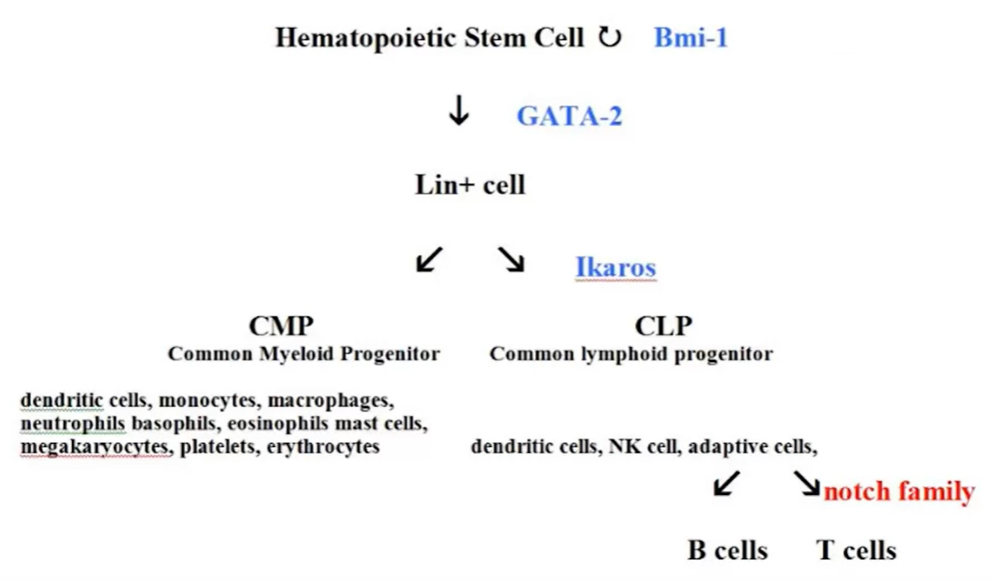
\includegraphics[scale=0.5]{2.2.1.png}
\end{center}
\end{itemize}
2.3\quad \textbf{Myeloid Granulocytes}
\begin{itemize}
\item \concept{Granulocytes} have granules and funky-looking nuclei.
\begin{itemize}
	\item \concept{Neutrophil}:
	\begin{itemize}
		\item Initial response to a threat.
		\item Strongly phagocytic, typically only lives for a day.	
		\item Multi-lobe nucleus.
		\item Granules are both acidic and basic.
		\item Has FC receptors that binds the antibody stems and targets threats.
	\end{itemize}
	\item \concept{Basophil}:
	\begin{itemize}
		\item Complex C-shaped nucleus.
		\item Not phagocytic.
		\item Part of the response to worms and environmental threats.
		\item Granules have C-shaped nucleus.
		\item Has FC receptors that hold E-class antibodies and go looking for antigen.
	\end{itemize}
	\item \concept{Mass cell}:
	\begin{itemize}
		\item Tends to stay at one location.
		\item Has lots of granules with histamine.
		\item Signals running nose, mucus production, and itching if has an allergic response.
		\item Nucleus has no lobes.
		\item Works with basophils to respond to worms and environmental pollutants.
		\item Has FC receptors that hold E-class antibodies and go looking for antigen.
	\end{itemize}
	\item \concept{Eosinophil}:
	\begin{itemize}
		\item Has a bilobed nucleus.
		\item Granules are red as they are staining with eosin red and acidic stain.
		\item Also attacks worms.
		\item Weakly phagocytic, most of the time secretes substances from those red staining granules at the warms.
	\end{itemize}
\end{itemize}
\item \concept{Hygiene hypothesis} states that early childhood exposure to particular microorganisms protects against allergic diseases by contributing to the development of the immune system.
\end{itemize}
2.4\quad \textbf{Myeloid Antigen Presenting Cells}
\begin{itemize}
\item Myeloid antigen presenting cells:
\begin{itemize}
	\item \concept{Monocyte}:
	\begin{itemize}
		\item Makes lot of inclusions and other molecules important in hydrolyzing pathogens, breaking them up, and using them to alert $\mathrm{T_H}$ cells.
		\item Not only phagocitize but also reach out and attempt to transmit information or grab pathogens.
		\item Mobile and has active surface, strongly phagocytic.
	\end{itemize}
	\item \concept{Sentinel Dendritic Cell}:
	\begin{itemize}
		\item First to present an antigen to naive $\mathrm{T_H}$ cells.
		\item Gatekeepers that decide whether or not a $\mathrm{T_H}$ cell will respond to a new antigen.
		\item Not migrating but lying in wait in a tissue to phagocytize antigen, digest it, and then present it to a $\mathrm{T_H}$ cell.
		\item Some belong to the lymphoid lineage.
	\end{itemize}
	\item \concept{Follicular dendritic cell}:
	\begin{itemize}
		\item Incredible number of extensions that can trap \concept{exosomes}, including particles and antigen-antibody complexes.
		\item Instructs B cells by giving them a chance to bind to a particular antigen-antibody complex and thus get some encouragement in their development.
	\end{itemize}
\end{itemize}
\end{itemize}
2.5\quad \textbf{Lymphocytes}
\begin{itemize}
\item B cells:
\begin{itemize}
	\item Developped in the bursa of Fabricius, which is the dorsal wall of the cloaca (common exit) of both the digestive and urogenital system of the bird. 
	\item Has membrane-bound antibody.
	\item Has class II MHC molecules, part of its their way of communicating with $\mathrm{T_H}$ cells.
	\item When stimulated to divide and develop and secrete antibodies, it becomes much larger and its protein synthesis apparatus will be up-regulated. 
\end{itemize}
\item T cells:
\begin{itemize}
	\item Either becomes \concept{cytotoxic} ($\mathrm{T_C}$) cell or \concept{helper} ($\mathrm{T_H}$) cell. $\mathrm{T_C}$ has CD8 and $\mathrm{T_H}$ has CD4. 
	\item $\mathrm{T_H}$ cells are quite diverse, including $\mathrm{T_H}1$, $\mathrm{T_H}2$, $\mathrm{T_{reg}}$, $\mathrm{T_H}17$, etc.
\end{itemize}
\item NK cells:
\begin{itemize}
	\item Many granules and a round nucleus.
	\item Has a trident of Fas ligand (FASL) that up-regulate apoptosis of the cell it sticks into.
	\item If it synapses with a rogue cell or viral-infected or cancerous cell, it has a lot of ammunition in the form of granzymes (serine proteases promoting cytotoxicity of rogue cells) and perforin (glycoprotein responsible for pore formation in cell membranes) that help to break up the cell and send it into asbestosis.
	\item Has MHC1\footnote{\concept{Major Histocompatibility Complex (MHC)} is a large locus on vertebrate DNA containing a set of closely linked polymorphic genes that code for cell surface proteins essential for the adaptive immune system.} regulator that down-regulates to stop from attacking.
	\item Has FC receptor so that if it finds antibodies stuck in the surface of a cell, it will attack the cell.
	\item In a $\mathrm{T_C}$ cell, the MHC receptor will recognize foreign antigen on MHC1 and attack the cell. If a virus down-regulates the production of MHC so that a $\mathrm{T_C}$ cell cannot be alerted to the presence of foreign antigen, NK cells attack it as well. This process is an innate response.
\end{itemize}
\end{itemize}
2.6\quad \textbf{Primary Organs}
\begin{itemize}
\item Three primary lymphoid organs: bursa, bone marrow and thymus.
\begin{itemize}
\item Bone marrow:
\begin{itemize}
	\item Produces most of the immune cells.
	\item Bone marrow has lots of fat that sends out signals that regulate hematopoiesis.
	\item Produces lymphoid cells.
	\item NK cells arise here and B cells rearrange their genes as part of their development.
	\item T cells start out here and migrate into the thymus to rearrange their genes.
	\item Primarily the femur\footnote{Thigh bone.}, humerus\footnote{Bone of the upper extremity.}, arm bones, hip bones, and sternum\footnote{T-shaped vertical bone that forms the anterior portion of the chest wall centrally.} that do the production of most of blood cells.
\end{itemize}
\item Thymus:
\begin{itemize}
	\item Rearrangement site for the T cells.
	\item Has a cortex (outer layer) and medulla (inner layer). 
	\item T cells start from the cortex. T cell progenitors come in in a relatively undifferentiated state. Then,
	\begin{itemize}
	    \item Rearranging genes occur. If no productive rearrangement is derived, the cell dies off.
		\item They undergo a positive selection in the cortex to make sure they can identify antigen on an MHC molecule. If so, they migrate towards the medulla.
		\item They undergo a negative selection in the medulla to get rid of T cells that recognize our own self antigens to prevent auto-immune diseases. 
	\end{itemize}
	Cells pass the three tests leave the circulation and head out to the secondary lymphoid organs to coordinate your immune response, and cells do not pass any of the test will die. Over 95\% of the cells undergo apoptosis as part of this process.
\end{itemize}
\end{itemize} 
\end{itemize}
2.7\quad \textbf{Secondary Organs}
\begin{itemize}
\item The secondary organs of the immune system form an interconnected surveillance system where the immune cells gather and exchange information, including the fluid, vessels and nodes.
\item Circulation involves both the blood vessel (round trip) and the lymph (one-way from the organs out). The plasma from the blood filters into the tissues carrying the proteins, only the lymphoid cells crossover but not the blood cells or myeloid cells.  
\item The lymphatic system picks up fluid throught the body. This drained interstitial fluid from tissues picking up lots of information is gathered up and filtered through the lymph nodes where the antigen is trapped and acted on. Eventually, these vessels grow into larger ones that in turn empty into\footnote{Flows into.} the thoracic duct, left subclavian vein, and then the heart to rejoin the blood circulation.
\item The lymph system also extends into the head, named as the \concept{meningeal system}. It connects with the deep cervical or neck lymph nodes. It lies between the dura mater and the meninges outside the brain and between the meningial arteries and the dural sinuses, which are the veins. The sagittal sinus over the top of the head, transverse sinuses runnning along the side, a lymph vessel is buried in there. It will divide into two transverse branches that contains valves only in the skull, leading out to the cervical lymph nodes. 
\item Fluids come into a lymph node and come out from the efferent vessel. The cortex of a lymph node holds the follicles and the B cells, the power cortex refers to the structure below the cortex, and the medulla sits inside.
\item B cells activated by antigen are to wind up in follicles. The germinal center is where the B cells develop in response to signals from the follicular dendritic cells, $\mathrm{T_H}$ cells, and macrophages will clean up the debris. B cells learn how to bind more tightly to the particular pathgenic antigen here.
\end{itemize}
2.8\quad \textbf{Other Secondary and Tertiary Organs}
\begin{itemize}
\item The lymph nodes, spleen, and gut mucosa are all secondary lymphoid organs. \begin{itemize}
	\item Spleen:
	\begin{itemize}
		\item Lies above the abdomen.
		\item Filters and monitors blood but not lymph.
		\item Has red pulp tissue where the macra fascias recycle old red blood cells.
		\item Has white pulp tissue where T cells participate in immune surveillance.
		\item Has a marginal zone that has B cells in follicles.
	\end{itemize}
	\item \concept{Mucosal Associated Lymphoid Tissue (MALT)} is a collection of tissues including \concept{Bronchial Associated Lymphoid Tissue (BALT)}, \concept{Nasal Associated Lymphoid Tissue (NALT)}, and \concept{Gut Associated Lymphoid Tissue (GALT)}.
	\item The tonsils, appendix, and Peyer's patches (bunch of follicles) in the intestine of some animals also participate in the activation of B cells.
	\item GALT:
	\begin{itemize}
		\item Picks up antigens from the lumen and transports into a developping follicle. Similar in aforementioned other issues.
		\item M cell is sequestering a bunch of immune function cells to facilitate information flow.
	\end{itemize}
\end{itemize}
\item The skin forms a tertiary organ:
\begin{itemize}
	\item Made up of the epidermis, epithelial tissue that sits on a basement membrane, and dermis.
	\item The epidermis derives from embryonic ectoderm, and the dermis derives from embryonic mesoderm. The skin is produced by combining cells from two different tissue layers. It secrets lots of commounds to protect us from pathogenic attack.
	\item Keratinocytes are epithelial cells that upon death retains the keratin and helps to make the skin waterproof. They also express MHC2 and present antigen to T cells. Setenal dendritic cells phagocytizes antigens here as well that can leave the epidermis and go off and look for T cells someplace else.
	\item There is a speical kind of T cells reside in the epidermis and other mucosal tissues that have special receptors. They have built-in quasi-innate recognition for the possible dangerous organisms.
\end{itemize}
\end{itemize}
2.9\quad \textbf{Final Issues}
\begin{itemize}
\item \concept{Apoptosis} is a controlled way of killing off a cell and disposing of the contents.
\item \concept{Necrosis} means a cell swelling, breaking open, spilling its guts, and causing inflammaton.
\end{itemize}
\end{document}
